\documentclass[aspectratio=169,shownotes]{beamer}
\usepackage{graphicx} 
\usepackage[]{tikz}
\usepackage{tabularx}
\usepackage[normalem]{ulem}
\usepackage{hyperref}
\usepackage{forest}


\title{Studieren im Digitalen Zeitalter \\\small Tools und Methoden\\ V0.1}
\author{Florian Rössing}
\date{\today}

\definecolor{folderbg}{RGB}{255,160,0}
\definecolor{folderbody}{RGB}{255,202,40}
\def\Size{4pt}
\tikzset{
  folder/.pic={
    \filldraw[rounded corners=0.3pt,color=folderbg](1pt,0.5*\Size-1pt) rectangle (1pt+0.4*9/6*\Size,0.5*\Size+1pt);  
    \filldraw[rounded corners=0.3pt,color=folderbody](1pt,-.5*\Size) rectangle (9/6*\Size+1pt,.5*\Size);  
    %\filldraw[](-\Size,-\Size) rectangle (\Size,\Size);
  }
}

\begin{document}

\maketitle

\section{Einführung}
\begin{frame}{Ich}
    Kurzer Lebenslauf und Motivation
\end{frame}

\begin{frame}{Worüber rede ich?}
\tableofcontents[sectionstyle=show,subsectionstyle=show/hide]
\end{frame}

\subsection{Anforderungen von Studenten}
\begin{frame}{Übersicht}
Was sind klassische Arbeiten eines Studenten?
    \begin{itemize}
        \item Mitschreiben
        \item Aufgaben bearbeiten
        \item Quellen sichten
        \item Präsentieren
        \item Kollaborieren     
        \item[$\Rightarrow$] Wissen ansammeln und teilen
        \item[$\Rightarrow$] \sout{Wissen} Daten ansammeln und teilen   
    \end{itemize}
\end{frame}
\note{Welche Art von arbeiten erledigen studenten regelmäßig?
Am Ende dient alles dem lernen, dem erlangen von Wissen!
Wissen ist auch nur eine Art von Daten!}

\begin{frame}{Wie hab ich es gemacht?}
    \begin{tabularx}{\linewidth}{ll}
        Mitschriften & Papier, Tablet \\
        Abgaben, Übungen & Papier\\
        Hausarbeiten, Thesis & \LaTeX\\
        Präsentationen & Powerpoint, \LaTeX\\
        Kommunikation & WhatsApp\\
        Teilen von Unterlagen & Dropbox (später Sciebo)\\                
    \end{tabularx}
    \pause
    \begin{tikzpicture}[overlay, remember picture]
        \node[anchor=south east] at ([shift={(-2.5cm,4cm)}]current page.south east) {
\includegraphics[width=3cm]{graphics/Meine_Mitschriften.jpg}};
        \pause
        \node[anchor=south east] at ([shift={(-2cm,3cm)}]current page.south east) {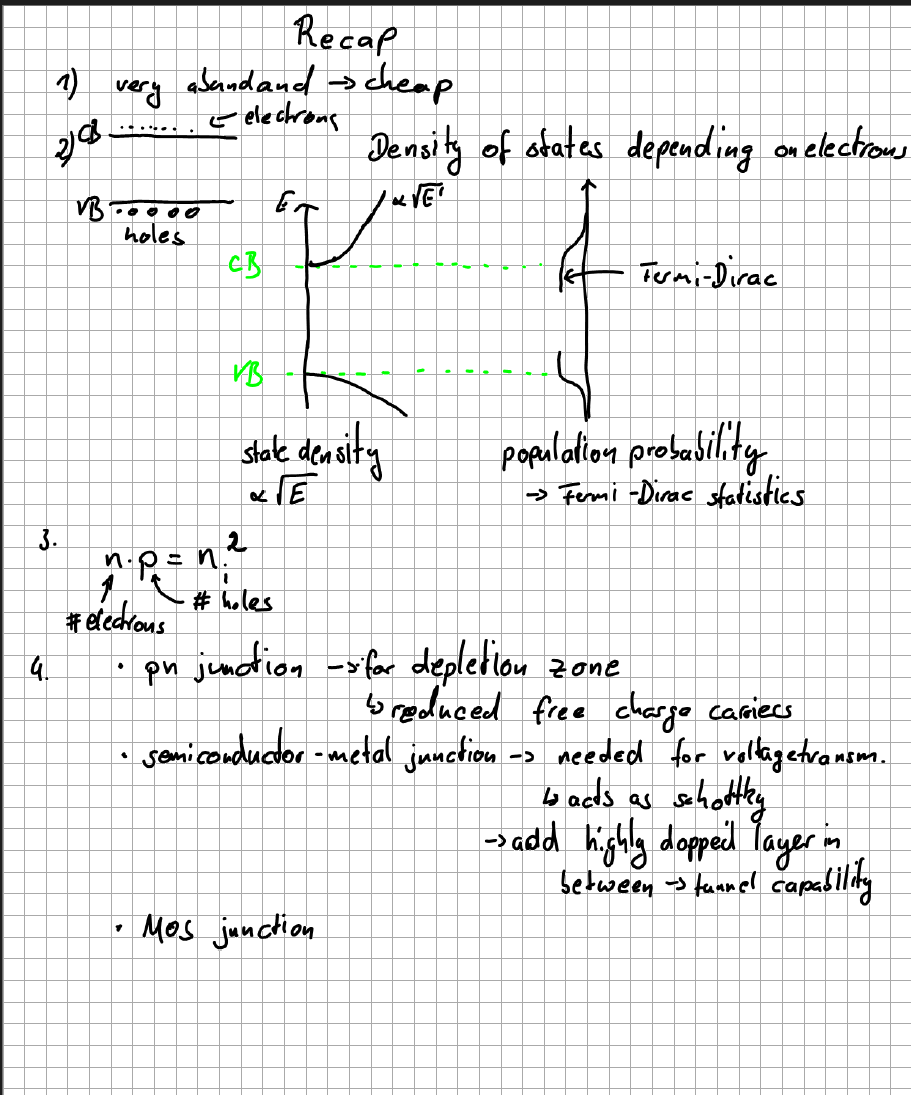
\includegraphics[width=3cm]{graphics/Meine_Mitschriften_Tablet.png}};
        \pause
        \node[anchor=south east] at ([shift={(-1.5cm,2cm)}]current page.south east) {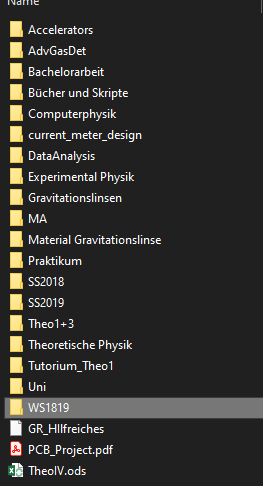
\includegraphics[width=3cm]{graphics/Meine-Unterlagen.png}};
        \pause
        \node[anchor=south east] at ([shift={(-2.5cm,4cm)}]current page.south east) {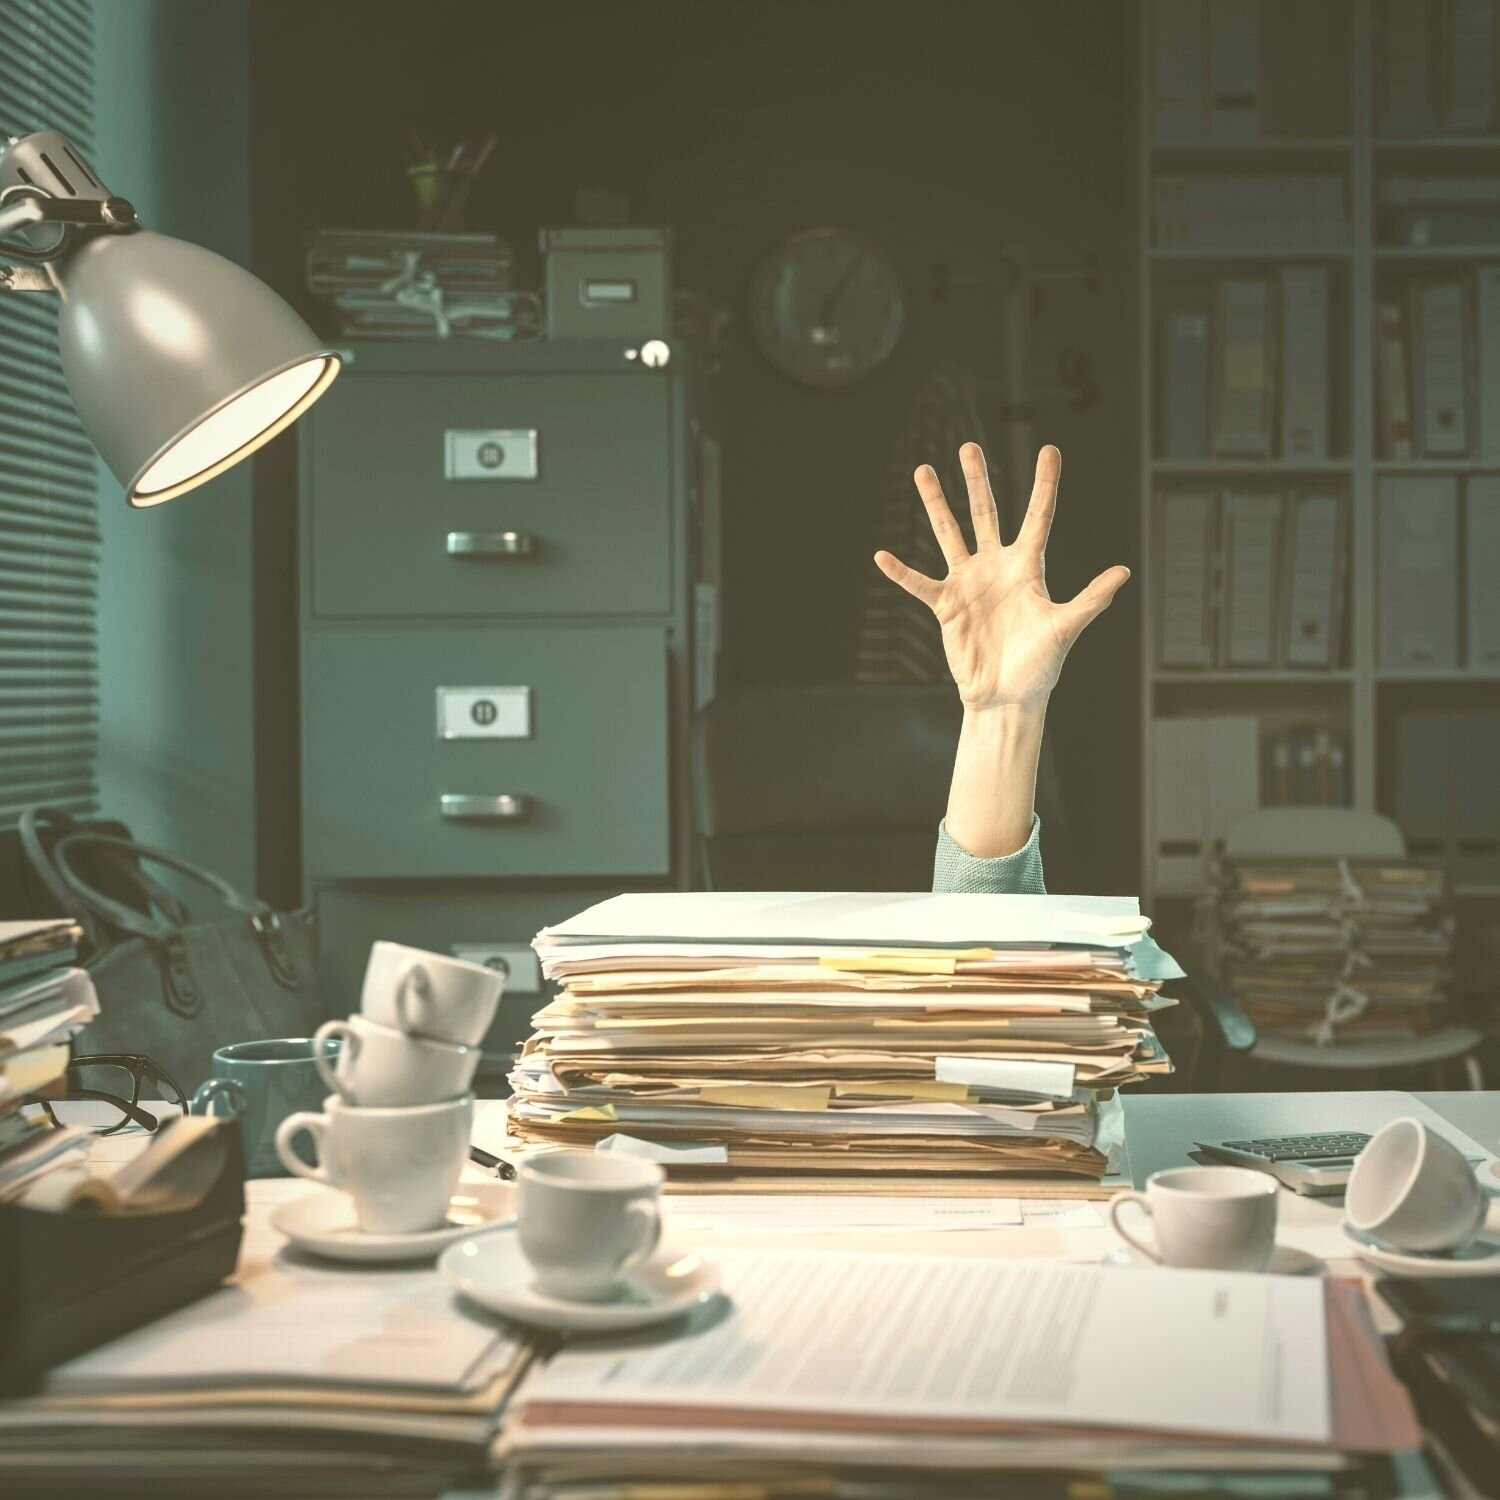
\includegraphics[height=4cm]{graphics/overwhelmed_student_2.jpg}};
    \end{tikzpicture}
    \pause
    \vspace{1cm}
\end{frame}
\note{
        \begin{enumerate}
        \begin{bf}
        \item Welche Formate eignen sich für meine Notizen?
        \item Wie organisiere ich meine Notizen so, dass ich nicht im Chaos versinke?
        \item Wie kann ich mit meinen Komilitonen zusammenarbeiten und unterlagen teilen?
        \end{bf}
\end{enumerate}}



\section{Ausgewählte Tools}


\subsection{Mitschriften}
\begin{frame}
    \Huge
    \centering
    Legt euch ein System für Notizen zu!

\end{frame}

\begin{frame}{Aber welches?} 
    \begin{block}{}
        Die einfache Antwort zuerst:
    \end{block}
    \begin{tikzpicture}
        \node[anchor=south west] at (0,2) {
\includegraphics[width=3cm]{graphics/Logos/GoogleWorkspace.jpeg}};
        \node[anchor=south west] at (3,1) {
\includegraphics[width=3cm]{graphics/Logos/Office365.png}};
        \node[anchor=south west] at (6,3) {
\includegraphics[width=3cm]{graphics/Logos/Evernote.jpeg}};
        \node[anchor=south west] at (9,2) {
\includegraphics[width=3cm]{graphics/Logos/Notion.jpeg}};
    \end{tikzpicture}
    \pause
    \begin{block}{}
        \centering\large Es muss zu eurem Stil passen!    
    \end{block}
\end{frame}
\note{Search, Cloud, Collab, Meetings, Local, conversion\\}

\begin{frame}{Die schwere Antwort: Bastelt euer eigenes System}
\pause
\begin{block}{Die FAIR Prinzipien}
    \begin{itemize}
        \setlength{\itemindent}{-2em}
        \item[] \textbf{F}indable - Auffindbar
        \begin{itemize}
            \item Eure Daten sollten leicht zu durchsuchen sein
            \item Eure Daten sollten gut strukturiert sein
        \end{itemize}
        \item[] \textbf{A}ccessible - Zugänglich
        \begin{itemize}
            \item Ihr solltet jederzeit Zugang zu euren Daten haben
            \begin{itemize}
                \item Habt immer eine lokale Kopie!
            \end{itemize}
        \item Macht eure Notizen auch euren Komilitonen zugänglich
    \end{itemize}
        \item[] \textbf{I}nteroperable - Interoperabel
        \begin{itemize}
            \item Verwendet gängige Dateiformate
            \item Stellt eure Quellen offen, nicht nur PDFs
            \item Sucht euch Tools die ihr verbinden könnt
        \end{itemize}
        \item[] \textbf{R}eusable - Wiederverwendbar
        \begin{itemize}
            \item Ihr solltet eure Unterlagen auch später noch zu rate ziehen können
        \end{itemize}
    \end{itemize}
\end{block}
\end{frame}


\begin{frame}[t]{DIY:}
\begin{columns}[t]   
    \begin{column}{0.5\textwidth}
    {\Large Notizen:\\}
    \begin{tikzpicture}
        \def\width{1cm}
        \node[anchor=north west] at (0,0) {
\includegraphics[width=\width]{graphics/Logos/Obsidian.png}};
        \node[anchor=north west] at (\width,0) {
\includegraphics[width=\width]{graphics/Logos/Joplin.png}};
        \node[anchor=north west] at (0,\width) {
\includegraphics[width=\width]{graphics/Logos/OneNote.jpeg}};
        \node[anchor=north west] at (\width,\width) {
\includegraphics[width=\width]{graphics/Logos/Word.jpeg}};
        \end{tikzpicture}
        \begin{enumerate}
            \item Verfügbar auf allen Geräten
            \item 
            \item Dateien übergreifende Suche
            \item Notizen Verknüpfen
            \item Verknüpfungen zu Quellen herstellen
        \end{enumerate}  
\end{column}
\begin{column}{0.5\textwidth}
    \Large Cloud:\\
    \begin{tikzpicture}
        \node[anchor=south west] at (0,2) {
\includegraphics[width=2cm]{graphics/Logos/Sciebo.jpeg}};
        \node[anchor=south west] at (0,4) {
\includegraphics[width=2cm]{graphics/Logos/Dropbox.jpeg}};
    \end{tikzpicture}
    \begin{enumerate}
        \item Sollte möglichst wenig kosten
        \item Speicherplatz 10 bis 50GB ausreichend
        \item 
    \end{enumerate}  
\end{column}        
\end{columns}
\end{frame}
\note{Ihr werdet immer eine Software brauchen, in der ihr Notizen anlegen könnt.
Word ist ein klassiker, aber nicht optimal für notizen.
OneNote ist ebenfalls von Microsoft, ist sehr flexibel, aber verwendet kein gängiges Format.
Joplin und Obsidian sind beides Tools die auf Markdown basieren.
Zusätzlich zu Notizen, müsst ihr die natürlich auch irgendwo Speichern, zusammen mit euren anderen Materialien.
Eine Cloud Lösung ist dafür ideal.
Dropbox ist eine der älteren und verbreiteten Lösungen. Sciebo ist eine alternative die von fast allen Universitäten angeboten wird. 
}

\begin{frame}[t]{Dateien Ordentlich ablegen}
\begin{columns}
    \begin{column}{0.5\textwidth}
        \vspace{-8cm}
        \begin{block}{Ein paar Grundregeln}
            \begin{itemize}
                \item Überlegt euch eine Struktur. 
                \item Schreibt die auf. Gute Angewohnheit: Eine ReadMe in den Top Ordner legen.
                \item Versucht möglichst wenige Ordner Level zu haben.
            \end{itemize}     
        \end{block}        
        \vfill   
    \end{column}
    \begin{column}[t]{0.35\textwidth}
        \begin{forest}
            for tree={
              font=\ttfamily,
              grow'=0,
              child anchor=west,
              parent anchor=south,
              anchor=west,
              calign=first,
              inner xsep=7pt,
              s sep=1pt,
              edge path={
                \noexpand\path [draw, \forestoption{edge}]
                (!u.south west) +(2pt,0) |- (.child anchor) pic {folder} \forestoption{edge label};
              },
              file/.style={edge path={\noexpand\path [draw, \forestoption{edge}]
                (!u.south west) +(7.5pt,0) |- (.child anchor) \forestoption{edge label};},
                inner xsep=2pt,inner ysep=0pt,font=\small\ttfamily
                     },
              before typesetting nodes={
                if n=1
                  {insert before={[,phantom]}}
                  {if n=3 
                  {insert before={[,phantom]}}
                  {}
                  }                
              },
              fit=band,
              before computing xy={l=15pt},
            }  
          [SS24
                [ReadMe.txt,file]
                [Grundlagen 1
                    [SW1
                        [VL.pdf,file]
                        [Übung.pdf,file]
                    ]
                    [SW2]
                ]
                [Nebenfach 1
                    [VL
                       [VL1.pdf,file]
                       [VL2.pdf,file]
                    ]
                    [Übungen
                        [Ü1.pdf,file]
                        [Ü2.pdf,file]
                    ]
                ]
            ]
          \end{forest}
    \end{column}
\end{columns}
   

\end{frame}

\subsection{Literatur}
\begin{frame}{Literatur Recherche}
    \begin{columns}[t]
        \begin{column}{0.29\textwidth}
            \vspace*{-0.1\textheight}
            \begin{figure}[t]
                
\includegraphics[height=0.8\textheight]{graphics/LiteraturChaos.jpeg}         
            \end{figure}
        \end{column}        
        \begin{column}{0.69\textwidth}
            \begin{itemize}
                \item Google, \href{https://scholar.google.com/}{Google Scholar}
                \item \href{https://www.connectedpapers.com/}{Connected Papers}
                \item \href{https://elicit.com/}{Elicit}
                \item ChatGPT
                \item Eure Uni Bibliothek!
            \end{itemize}           
            \vspace{1cm}            
            \begin{itemize}
                \item \textcolor{lightgray}{libgen.ist}
                \item \textcolor{lightgray}{scihub.st}
            \end{itemize} 
        \end{column}        
    \end{columns}  
\end{frame}


\begin{frame}{Literatur Verwaltung}
    \begin{columns}[t]
        \begin{column}{0.29\textwidth}
            \vspace*{-0.1\textheight}
            \begin{figure}[t]
                
\includegraphics[height=0.8\textheight]{graphics/LiteraturChaos.jpeg}         
            \end{figure}
        \end{column}        
        \begin{column}{0.69\textwidth}
            \begin{itemize}
                \item Citavi
                \item Zotero
                \item Mendeley
            \end{itemize}           
        \end{column}        
    \end{columns}    
\end{frame}

\begin{frame}{Zettelkasten}
    Eine Methode gelerntes zu Dokumentieren und Organisieren
    - Brecht wissen herunter auf atomare kleine zettelchen
    - linkt nahe gelegenes wissen 
\end{frame}

\begin{frame}{Lernkarten mit Anki}
    Einfaches Erstellen von Lernkarten
    
\end{frame}

\begin{frame}{Time Boxing}
    Kalender   
    
    Pomodoro
\end{frame}

\begin{frame}{ToDo Listen}
    Todolisten
\end{frame}

\begin{frame}{Rechtschreibung und Gramatik}
    Gramarly
    DudenMentor
    LanguageTool
\end{frame}

\begin{frame}{Kommunikation}
    \begin{itemize}
        \item WhatsApp
        \item Slack
        \item Discord
        \item Matrix        
    \end{itemize}
\end{frame}

\begin{frame}{Ein kurzer Google Cheat Sheet}
    \begin{itemize}
        \item \textit{site:} beschränke die Suche auf eine Webseite
        \item \textit{filetype:} sucht nach Dateien vom Typ
        \item \textit{""}  Muss im Ergebnis vorkommen
        \item \textit{-} Darf nicht im Ergebnis vorkommen
        \item \textit{AND,OR} Logisches Verknüpfen von Suchbegriffen
    \end{itemize}
\end{frame}


\section{Addendum}
\subsection{Günstige Hardware}
\begin{frame}{Ein Laptop für den schmalen Euro}
    
\end{frame}

\subsection{Support}

\begin{frame}{Das HRZ}
    
\end{frame}

\begin{frame}{Online Communities}
    \begin{tabularx}{\linewidth}{ll}
        Reddit & Communities zu methoden, Fächern und Tools mit vielen hilfsbereiten Mitgliedern\\
        YouTube & Muss ich glaube ich nicht erklären\\
        Discord Server & Hard zu finden, aber ein guter Interaktionsort für spezifische Themen.\\

    \end{tabularx}
\end{frame}
\end{document}
